\begin{frame}{Lysåben vegetation / arronderinger}

\small

\begin{columns}[T]

\begin{column}{0.58\textwidth}

\textbf{Regler for lysåben vegetation / arronderinger:}

\begin{itemize}[]
\item \textbf{Arrondering}: Fx afrunding af hjørner i marken
\item Kan bestå af: græsarealer, naturlig vegetation (udyrket areal) og/eller vildtstriber
\item \textbf{Græsarealer}: Primært græs, plejet kort via afgræsning eller høslet
\item \textbf{Vildtstriber}: Tilsået med vildt- og bivenlige plantearter
\item Tilladte arter: Alle ikke-traditionelle afgrøder i renbestand
\end{itemize}

\vspace{0.05em}

\textbf{Gavner arter:}

\footnotesize
Agerhøne, fasan, hare, rådyr, sanglærke, vibe, gul vipstjert, 
rødrygget tornskade, gulspurv, markpiber, vilde bier, humlebier, 
dagsommerfugle, svirrefluer, rovbiller, græshopper, markmus, 
pindsvin, lækat, flagermus, musvåge, tårnfalk

\end{column}

\begin{column}{0.40\textwidth}
\centering
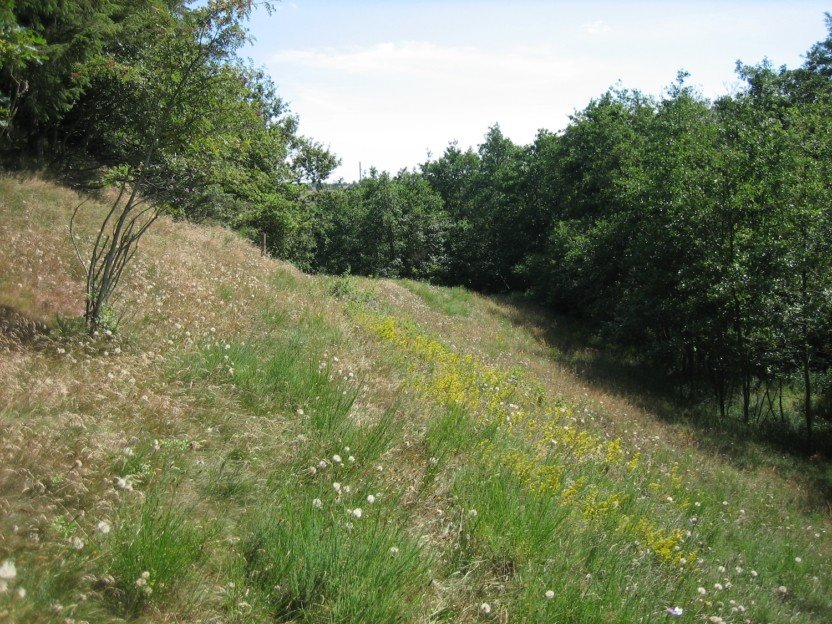
\includegraphics[width=\textwidth]{Billeder/Vildtforvaltning/biotopplantiltag/lysåben.jpg}
\end{column}

\end{columns}

\end{frame}